\section{Experiments\label{exp}}
\subsection{Evaluation Setup}
\subsubsection*{TestBed} We evaluated SharpView on a PC equipped with Nvidia 2080Ti 11GB GPU, Intel i5-12400 CPU and 32GB RAM. 

\subsubsection*{Baselines} We compare SharpView (referred to as Sharp.) against three baselines: random (referred to as Rand.), maximal distance (referred to ass MDist.) and prediction-based NBV (referred to as Pred.).
Rand. is a pure randomized strategy.
MDist. maximizes the distance between selected view to the view from the training dataset.
Pred. is a prediction-based method that trains an extra head on the MLP decoder of the grided view synthesis pipeline
following the patterns of loss functions commonly used in these methods~\cite{shen_stochastic_2021,jin_neu-nbv_2023,ran_neurar_2023,avidan_activenerf_2022}: 
\begin{equation}
    L = \frac{1}{R} \sum_{r=0}^R  \big ( \log \sigma_r + \frac{(c_r-\hat{c}_r)^2}{\sigma_r^2} \big )
    \label{uncertainty}
\end{equation}
where $R$ is the number of pixels in an input image, $\sigma_r$ is the standard deviation prediction from the extra model head, $c_r$ is the predicted rgb value, and $\hat{c}$ is the groundtruth rgb measurement.

\subsubsection*{Workload}
We choose DirectGO~\cite{sun_direct_2022} as the grided view synthesis pipeline for our evaluation, which features a implicit voxel grid representation of the 3D scene and short convergence time within minutes, compared with the convergence time of days using the non-grided counterparts.
It also achieves comparable resulting view synthesis accuracy.
We follow DirectGO to use PSNR, SSIM~\cite{1284395}, and LPIPS~\cite{8578166} as the metrics to compare the view synthesis accuracy among SharpView and the baselines.

\subsubsection*{Datasets}
We evaluate our approach on three different datasets. We configure the datasets mainly following the default setup of DirectGO~\cite{sun_direct_2022}. Synthetic-NeRF contains eight objects with realistic images synthesized by NeRF. Synthetic-NSVF contains another eight objects synthesized by NSVF. We follow the setup of these two datasets and set the image resolution to 800 $\times$ 800 pixels and set 100 views for training and NBV selection and 200 views for testing for each scene.
TanksAndTemples is a real-world dataset captured from large real-world 3D scenes with  1920 $\times$ 1080 image resolution. We set one-eighth of the images testing and the rest for training and NBV selection.

\subsubsection*{NBV Configuration}
We initialize the NBV procedure by training the grided view synthesis pipeline with a initial training dataset sized six views.
And the NBV procedure ceases after acquiring ten new views from the training dataset.
The six views are selected by randomly selecting the first view and then append the rest views with the same policy with MDist., so that all surfaces of the 3D scene are more likely to be covered at the initial stage.
After a view is appended to the training set, we retrain the grided view synthesis pipeline to avoid overfitting to the previous views in the training set and compute new NBV information gain estimation.
In the training procedure, we scale the default configuration of number of training iterations and learning rate decay from DirectGO~\cite{sun_direct_2022} by the ratio between the length of training set and the whole training dataset.
At the end of the NBV procedure, the view synthesis accuracy results are calculated and
we present below the results averaged over repeating the evaluation with three different seeds.
% The results below are averaged on the results evaluated with three different seeds.



\subsection{Quantitative Comparison}
We first qualitatively compare the view synthesis accuracy results under different NBV methods.
With the knowledge of loss space sharpness of each candidate views, SharpView managed to select views with more information gain from the candidate views as the NBV, and constantly outperformed the baselines in terms of PSNR, SSIM and LPIPS as shown in Table~\ref{nsvf}, ~\ref{nerf} and~\ref{tank}.

Note that while the results of Rand. and MDist. are comparable since they are both naive methods without any information gain estimation, Pred. constantly performed the worst, which means that Pred. tended to select views with less information gain in the grided view synthesis settings.
The possible reason for this phenomenon is two-fold.
First, the extra term and factor introduced in their loss function as in Equation~\ref{uncertainty} in additional to the mean square error may decrease the magnitude of the computed loss value and thus slow down convergence.
Second, the local latent codes in different cells are separately and imbalancedly trained, which means the supervision of certain cells can be weak, especially the less frequently visited and thus uncertain cells.
This results in that the frequently visited cells output low uncertainty (standard deviation of its rgb output $\sigma$) and less frequently visited cells output uncertainty of comparatively random values, severely interfering their NBV selection.



\begin{table*}[h!]
    \centering
    \caption{Results on Synthetic-NSVF. }
    \begin{tabular}{|c|c|c|c|c|c|c|c|c|c|}
        \hline
        \multirow{2}{*}{Methods} & \multicolumn{3}{c|}{Palace} &  \multicolumn{3}{c|}{Robot} &  \multicolumn{3}{c|}{Spaceship} \\ \cline{2-10}
         & PSNR$\uparrow$ & SSIM $\uparrow$& LPIPS $\downarrow$ & PSNR$\uparrow$ & SSIM $\uparrow$& LPIPS $\downarrow$& PSNR $\uparrow$& SSIM $\uparrow$& LPIPS $\downarrow$

         \\ \hline Rand.  & 27.841 & 0.884 & 0.084 & 25.777 & 0.949 & 0.047 & 26.181 & 0.944 & 0.05
         \\ \hline MDist.  & 27.56 & 0.879 & 0.082 & 25.357 & 0.946 & 0.049 & 25.805 & 0.942 & 0.05
         \\ \hline Pred.  & 26.111 & 0.849 & 0.118 & 23.454 & 0.929 & 0.070 & 24.049 & 0.928 & 0.073
         \\ \hline Sharp.  & $\bm{28.768}$ & $\bm{0.897}$ & $\bm{0.069}$ & $\bm{27.653}$ & $\bm{0.963}$ & $\bm{0.025}$ & $\bm{26.561}$ & $\bm{0.948}$ & $\bm{0.047}$
         \\ \hline
    \end{tabular}
    \label{nsvf}
\end{table*}

\begin{table*}[h!]
    \centering
    \caption{Results on Synthetic-NeRF. }
    \begin{tabular}{|c|c|c|c|c|c|c|c|c|c|}
        \hline
        \multirow{2}{*}{Methods} & \multicolumn{3}{c|}{chair} &  \multicolumn{3}{c|}{lego} &  \multicolumn{3}{c|}{ship} \\ \cline{2-10}
         & PSNR$\uparrow$ & SSIM $\uparrow$& LPIPS $\downarrow$ & PSNR$\uparrow$ & SSIM $\uparrow$& LPIPS $\downarrow$& PSNR $\uparrow$& SSIM $\uparrow$& LPIPS $\downarrow$

         \\ \hline Rand.  & 26.03 & 0.916 & 0.082 & 25.889 & 0.904 & 0.062 & 23.871 & 0.797 & 0.192
         \\ \hline MDist.  & 27.034 & 0.928 & 0.07 & 26.392 & 0.911 & 0.056 & 24.609 & 0.798 & 0.184
         \\ \hline Pred.  & 23.224 & 0.871 & 0.129 & 22.521 & 0.842 & 0.117 & 22.744 & 0.747 & 0.227
         \\ \hline Sharp.  & $\bm{28.573}$ & $\bm{0.936}$ & $\bm{0.049}$ & $\bm{27.133}$ & $\bm{0.919}$ & $\bm{0.047}$ & $\bm{25.116}$ & $\bm{0.805}$ & $\bm{0.171}$
         \\ \hline
    \end{tabular}
    \label{nerf}
\end{table*}


\begin{table}[h!]
    \centering
    \caption{Results on TanksAndTemple (Averaged across different scenes). }
    \begin{tabular}{|c|c|c|c|}
        \hline
        Methods & PSNR$\uparrow$ & SSIM $\uparrow$& LPIPS $\downarrow$ 

         \\ \hline Rand.  & 21.369 & 0.871 & 0.210
         \\ \hline MDist.  & 21.188 & 0.867 & 0.217
         \\ \hline Pred.  & 17.437 & 0.837 & 0.264
         \\ \hline Sharp.  & $\bm{22.674}$ & $\bm{0.879}$ & $\bm{0.200}$
         \\ \hline
    \end{tabular}
    \label{tank}
\end{table}

\subsection{Qualitative Comparison}
Here we present some details of the tested view synthesis results after the NBV procedure of each method for qualitative comparison, which shows that synthesized views with SharpView recovered finer details of the 3D scenes.


\begin{figure*}[ht!]
    \centering
      \begin{subfigure}{0.19\textwidth}
        \centering   
        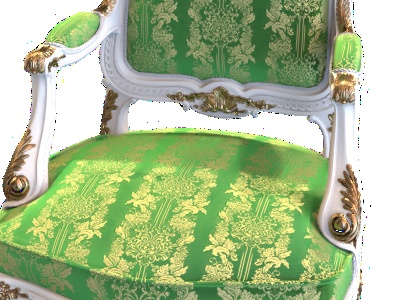
\includegraphics[width=\linewidth]{figs/gt_chair.jpg}
          \caption{groundtruth}
          \label{fig:sub1}
      \end{subfigure}   %      \hfill  % 这个\hfill指令为插入弹性长度的空白,看情况选择加不加。
      \begin{subfigure}{0.19\textwidth}
        \centering   
        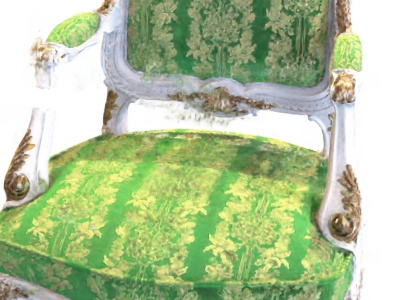
\includegraphics[width=\linewidth]{figs/random_chair.jpg}
          \caption{Rand.}
          \label{fig:sub2}
      \end{subfigure}
      \begin{subfigure}{0.19\textwidth}
        \centering   
        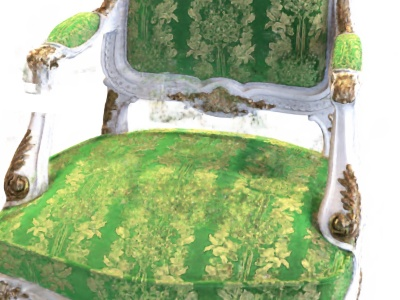
\includegraphics[width=\linewidth]{figs/max_dist_chair.jpg}
          \caption{MDist.}
          \label{fig:sub2}
      \end{subfigure}
      \begin{subfigure}{0.19\textwidth}
        \centering   
        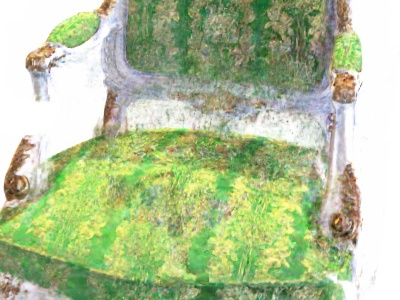
\includegraphics[width=\linewidth]{figs/uncertainty_chair.jpg}
          \caption{Pred.}
          \label{fig:sub2}
      \end{subfigure}
      \begin{subfigure}{0.19\textwidth}
        \centering   
        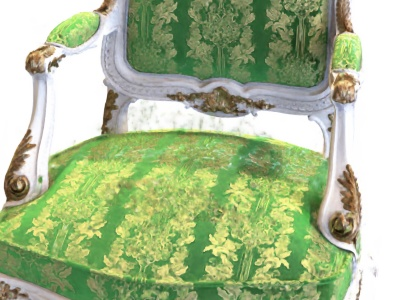
\includegraphics[width=\linewidth]{figs/sharpness_chair.jpg}
          \caption{Sharp.}
          \label{fig:sub2}
      \end{subfigure}
  \caption{
  \label{fig:total}
  Qualitative Comparison on Synthesis Nerf chair.
  }
\end{figure*}


\begin{figure*}[ht!]
    \centering
      \begin{subfigure}{0.19\textwidth}
        \centering   
        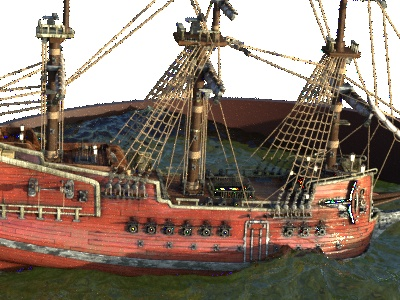
\includegraphics[width=\linewidth]{figs/gt_ship.jpg}
          \caption{groundtruth}
          \label{fig:sub1}
      \end{subfigure}   %      \hfill  % 这个\hfill指令为插入弹性长度的空白,看情况选择加不加。
      \begin{subfigure}{0.19\textwidth}
        \centering   
        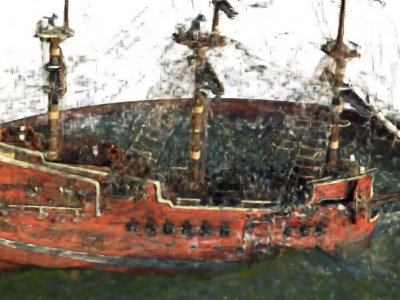
\includegraphics[width=\linewidth]{figs/random_ship.jpg}
          \caption{Rand.}
          \label{fig:sub2}
      \end{subfigure}
      \begin{subfigure}{0.19\textwidth}
        \centering   
        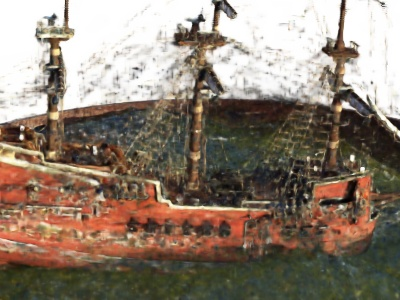
\includegraphics[width=\linewidth]{figs/max_dist_ship.jpg}
          \caption{MDist.}
          \label{fig:sub2}
      \end{subfigure}
      \begin{subfigure}{0.19\textwidth}
        \centering   
        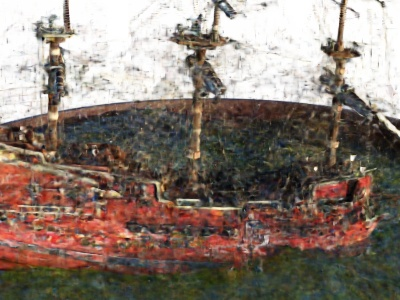
\includegraphics[width=\linewidth]{figs/uncertainty_ship.jpg}
          \caption{Pred.}
          \label{fig:sub2}
      \end{subfigure}
      \begin{subfigure}{0.19\textwidth}
        \centering   
        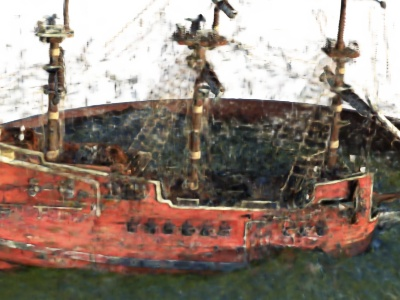
\includegraphics[width=\linewidth]{figs/sharpness_ship.jpg}
          \caption{Sharp.}
          \label{fig:sub2}
      \end{subfigure}
  \caption{
  \label{fig:total}
  Qualitative Comparison on Synthesis Nerf ship.
  }
\end{figure*}

\subsection{Discussion and Limitation}
Due to limited time budget, we did not make it to broadly and extensively evaluate SharpView and we are taking it as the future work.
Although we are motivated by the problems induced by grided view synthesis, the resulting algorithm and pipeline does not rely on the architecture or design of grided view synthesis, and we are curious about whether similar advantages can be achieved on other view synthesis architecture or even other domain of implicit rendering such as 3D reconstruction, which is also regarded as our future work.